\documentclass[runningheads]{llncs}

\usepackage{graphicx}
\usepackage{amsmath,amssymb}
\usepackage{booktabs}
\usepackage{hyperref}
\usepackage{tikz}
\usetikzlibrary{positioning,arrows.meta,calc}

\newcommand{\sayan}[1]{\textcolor{blue}{[Sayan: #1]}}

\begin{document}

\title{Abstract Rendering Toolkit for}
\author{Author Name}
\institute{Your Institution}

\maketitle

\begin{abstract}
    Abstract rendering over-approximates the set of images produced by uncertain poses and scenes, enabling end-to-end robustness claims for vision pipelines. We present \ART, a toolkit that turns this idea into a reproducible formal-verification workflow. Users describe a bounded subset of \(SE(3)\) as a tube of cylinders along a nominal trajectory (JSON) and provide scene, camera, and partitioning options in a short YAML file. \ART\ then (i) validates the pose tube, (ii) partitions pose/scene space anisotropically, (iii) runs abstract rendering on each cell and caches per-pixel bounds, and (iv) invokes a bound-propagation verifier (CROWN) on the cached abstract images, storing per-cell verdicts. The cached “AR” and “verification” dictionaries share keys, making failures traceable to their rendering evidence and eliminating reruns when models change. We demonstrate \ART\ on vision-based pose estimation for drone racing (GateNet) across four 3D Gaussian Splat tracks ($\approx$470k Gaussians each); a full verification sweep completes in $10–11$ hours on a single RTX 4070. All code, scenes, and scripts are released to support artifact evaluation and future verification research on vision-centric autonomy.
\end{abstract}

\section{Introduction}
\label{sec:introduction}

Certification of vision-based systems under semantic uncertainties is an important and challenging problem with applications in safety-critical domains such as automotive (vision-based lane keeping~\cite{yin2025certified,9852797} and emergency braking~\cite{yin2025certified}), avionics (vision-based navigation and landing~\cite{semerikov2025vision,santa2022nnlander,li2023refiningperceptioncontractscase}), and robotics (vision-based manipulation~\cite{hu2022robustness}). Semantic uncertainties refer to variations in the 3D scene and camera parameters that affect the rendered images, such as changes in object positions, lighting conditions, and camera viewpoints. Traditional robustness verification techniques for vision models primarily focus on pixel-level perturbations (e.g., adversarial attacks~\cite{szegedy2014intriguingpropertiesneuralnetworks,kurakin2017adversarialexamplesphysicalworld,madry2018towards,8294186,9614158}), which do not capture the rich set of semantic variations encountered in real-world scenarios.
With the emergence of 3D reconstruction techniques such as Neural Radiance Fields (NeRFs)~\cite{10.1145/3503250} and 3D Gaussian Splats (3DGS)~\cite{10.1145/3592433}, it has become possible to learn detailed 3D representations of scenes from images and render novel views. This not only enabled new ways of synthesizing training data for vision models and robotics simulators~\cite{falcon} but also opened up avenues for verifying vision models under semantic uncertainties by reasoning about the underlying 3D scenes and camera parameters.


Abstract rendering~\cite{AbstractRendering_Neurips2025} is a recently developed technique for over-approximating the set of all possible rendered images that can result from a set of camera poses and 3D scenes with semantic uncertainties. In a nutshell, abstract rendering takes as input a bounded set of camera poses---defined by interval pose matrices---and a set of scenes represented by 3D Gaussian spats (3DGS)~\cite{10.1145/3592433}, and propagates these sets through the standard 3DGS rendering algorithm to compute the output set of {\em abstract images}, which are represented by per-pixel color intervals or linear bounds. The key enabler for this technique is a set of piecewise linear relational abstractions for certain primitive nonlinear operations (such as matrix inverse and sorting-based summation) that appear in the rendering algorithm and careful engineering of the composition of these abstractions in the Crown~\cite{zhang2018efficient} bound propagation framework to ensure tightness of the final abstract images.

Previous work~\cite{AbstractRendering_Neurips2025,Habeeb-AbstractImages24} has demonstrated the feasibility  of abstract rendering in certifying the robustness of image processing models like classifiers and object detectors against {\em small ranges\/} of semantic purterbations, such as planar camera movements around a target object  and lighting changes. For larger-scale applications, such as verifying vision-based controllers operating in large scenes, abstract rendering needs to be integrated into a larger verification workflow that can efficiently specify, partition, and manage the large number of abstract rendering queries that arise in such settings.

\chenxi{updated below paragraph}

This paper introduces an open-source toolkit for abstract rendering tailored to the verification community. The toolkit provides a user-friendly interface for defining 3D scenes with semantic uncertainties, specifying camera parameters, and controlling variations in Gaussian-based scene representations. The main contributions of this work are as follows:

1) To the best of our knowledge, this is the first tool capable of verifying the robustness of a complete vision pipeline (Gaussian splatting + GateNet) in large-scale 3D scenes over 3-dimension pose space, supporting environments with up to 500k Gaussians while providing certifiable accuracy at the 10\,cm level.

2) We provide a flexible and modular infrastructure that enables researchers to systematically evaluate their methods on our dataset. Specifically, the framework allows users to: (i) explore different rendering algorithms on the same scene representation, (ii) apply and compare different abstraction methods using the same rendering pipeline and scene, and (iii) leverage our pre-tested scene data as a benchmark for reproducible evaluation. Together, these contributions offer both a first-of-its-kind verification tool and a practical benchmark for research in abstract rendering and pose estimation.

3) Compared with prior work~\cite{AbstractRendering_Neurips2025}, our approach supports a more general definition of planar motion by representing trajectories as sequences of waypoints, each associated with a local pose cell, enabling structured exploration of the pose space.

\section{Background: Rendering and Abstract Rendering}
\label{sec:background}

A  Gaussian Splat scene is defined by a collection of Gaussians in 3D space, and each Gaussian is $4$-tuple with a  mean position  $\mu_i \in \mathbb{R}^3$, a covariance shape matrix $\Sigma_i$, a color $c_i$, and an opacity $\alpha_i$. A rendering algorithm takes  a scene and a camera pose and computes the  color for each pixel in a 2D image as follows: (1) each Gaussian center \(\mu_i\) is transformed into the camera frame using the camera extrinsics; (2) the Gaussians are projected from camera coordinates to the 2D image plane via the camera intrinsics; (3) Gaussians are depth-sorted along the viewing direction; and (4) colors are blended in that order using a cumulative sum of products of colors and opacities. The blending implements volumetric compositing: closer, opaque Gaussians dominate a pixel; distant or transparent Gaussians contribute proportionally less.

Abstract rendering over-approximates every stage above with piecewise-linear relational bounds~\cite{AbstractRendering_Neurips2025}. Each geometric transform (world \(\to\) camera, camera \(\to\) image) and each per-pixel blend is replaced by a relation that encloses all possible function outputs for the given input sets of poses and scenes.
An abstract rendering-like algorithm for simpler mesh-based scenes was introduced~\cite{Habeeb-AbstractImages24}.


\section{Using the Abstract Rendering Toolkit}
\label{sec:art}

We will discuss the main components of the Abstract Rendering Toolkit (ART) using a running example of certifying the robustness of a GateNet~\cite{9636207} vision-based pose estimator for drone racing under pose and scene uncertainties.

\paragraph{Running example and scope.}
In this application, a drone equipped with a forward-facing camera must navigate through a sequence of gates in a racing arena. GateNet is a neural network that takes as input an RGB image from the drone's camera and outputs a 6-DoF {\em pose estimate} $\hat{y} \in SE(3)$ which includes the 3D position of the drone in the arena and its orientation (roll, pitch, yaw). This pose estimate is used by the drone's controller to adjust its flight path and successfully pass through the gates. Inaccuracies in the pose estimate can lead to collisions with the gates or failure to pass through them. For this example, we use $\ART$ for certifying GateNet's robustness over a user-provided bounded set $P \subset SE(3)$ of possible drone poses around a nominal trajectory that passes through the gates. Additionally, ART can also certify models considering semantic uncertainties in the scene, such as variations in gate colors or lighting conditions.


Figure~\ref{fig:art-workflow} summarizes the stages of the verifcation process using $\ART$ which are as follows: (1) User specifies the pose space $P$ in a JSON file and the scene file along with camera and algorithmic parameters in a YAML configuration file. (2) $\ART$ partitions $P$ into smaller cells $\{P_i\}$ and creates a dictionary of these pose cells. (3) For each pose cell $P_i$, $\ART$ performs abstract rendering to compute the corresponding abstract image $A_i$ and stores it in a dictionary. (4) Each abstract image $A_i$ is fed to GateNet using the CROWN~\cite{zhang2018efficient} verifier to obtain interval bounds on the predicted pose $\hat{Y}_i$, which are stored in a third dictionary.  Finally, (5) for each cell $P_i$, the predicted pose bounds $\hat{Y}_i$ are checked against the input pose cell $P_i$ (with a user-specified tolerance) to determine if GateNet is robust over that cell. In what follows, we describe each of these stages in more detail.

\begin{figure}
    \centering
    \includegraphics[width=0.45\textwidth]{figures/circle.png}
    \includegraphics[width=0.45\textwidth]{figures/abstract_viz_000000.png}
    \caption{\small Left: nominal trajectory (black) through blue racing gates. The user-defined input pose space $P$ is shown as a cyan tube. Right: {top-left} a sample image rendered in the 3DGS scene from a particular camera pose $p \in P$. Bottom-left and right images show the  abstract image corresponding to a cell $P_i \subseteq P$ that contains $p$ and is computed by our abstract rendering engine. Top-right \sayan{??}.}
\end{figure}

\begin{figure}[ht]
    \centering
    \resizebox{\linewidth}{!}{%
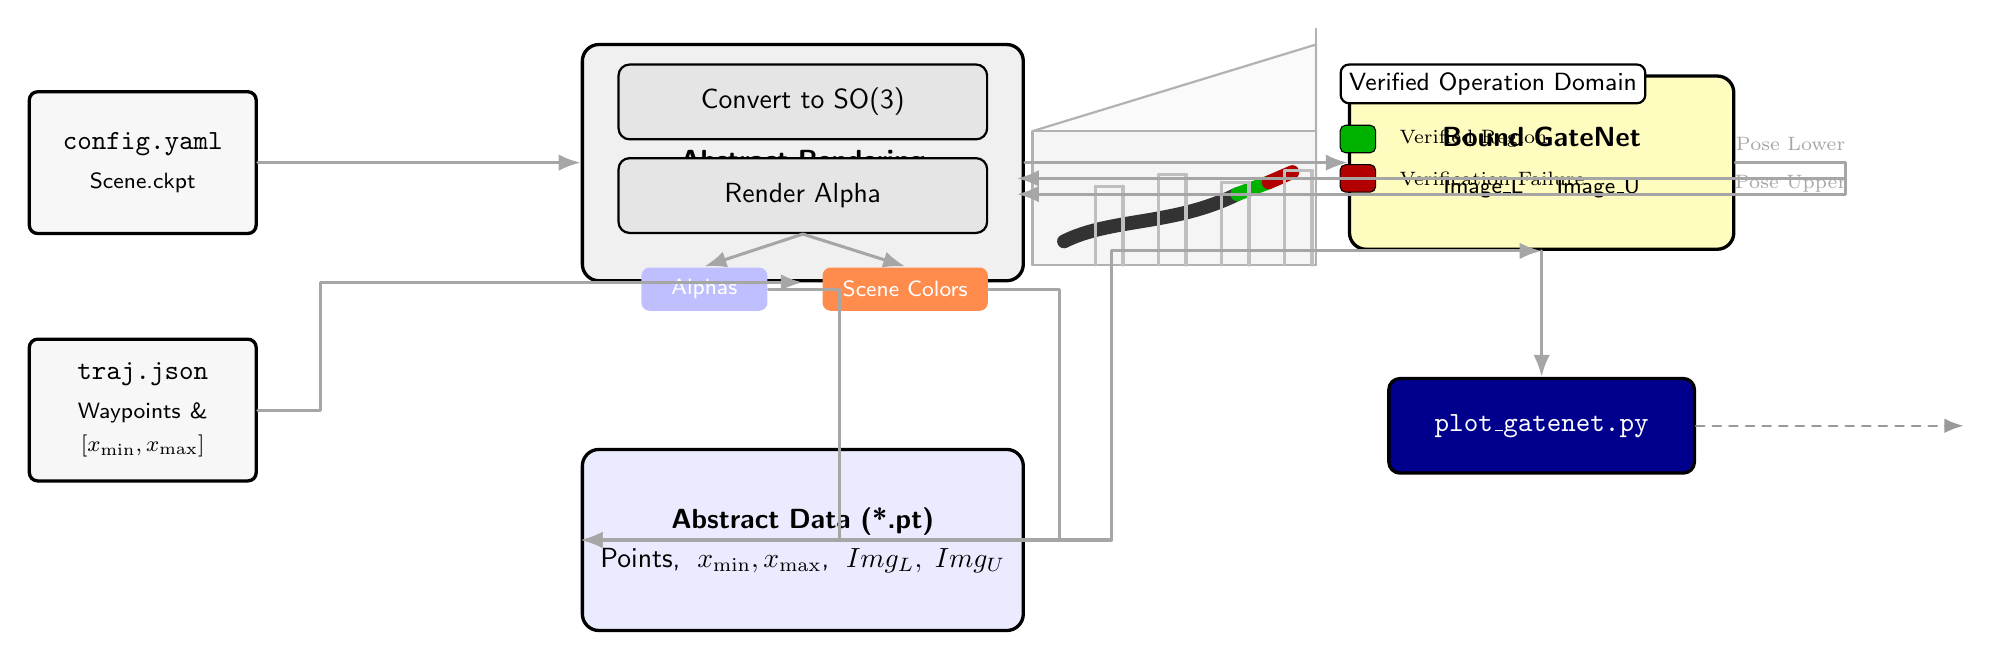
\begin{tikzpicture}[
    font=\sffamily,
    line join=round,
    line cap=round,
    >=Latex,
    node distance=1.4cm and 3.8cm,
    every node/.style={inner sep=4pt},
    filebox/.style={draw, rounded corners=3pt, fill=gray!6, very thick,
        minimum width=2.7cm, minimum height=1.8cm, text width=2.6cm, align=center},
    proc/.style={draw, rounded corners=6pt, fill=gray!12, very thick,
        minimum width=5.6cm, minimum height=3.0cm, text width=5.2cm, align=center},
    subproc/.style={draw, rounded corners=4pt, fill=gray!20, thick,
        minimum width=4.6cm, minimum height=0.95cm, text width=4.4cm, align=center},
    data/.style={draw, rounded corners=6pt, fill=blue!8, very thick,
        minimum width=5.6cm, minimum height=2.3cm, text width=5.2cm, align=center},
    model/.style={draw, rounded corners=6pt, fill=yellow!25, very thick,
        minimum width=4.8cm, minimum height=2.2cm, text width=4.6cm, align=center},
    script/.style={draw, rounded corners=4pt, fill=blue!55!black, text=white, very thick,
        minimum width=3.8cm, minimum height=1.2cm, text width=3.6cm, align=center},
    legendbox/.style={draw, rounded corners=2pt, minimum width=0.45cm, minimum height=0.35cm},
    callout/.style={draw, fill=white, rounded corners=3pt, thick, inner sep=3pt},
    dashedflow/.style={dash pattern=on 3pt off 3pt, line width=0.9pt, gray!80},
    flow/.style={-Latex, line width=1.1pt, gray!70}
]

% Inputs
\node[filebox] (config) {\texttt{config.yaml}\\[2pt]\footnotesize Scene.ckpt};
\node[filebox, below=1.3cm of config] (traj) {\texttt{traj.json}\\[2pt]\footnotesize Waypoints \& $[x_{\min},x_{\max}]$};

% Abstract rendering block
\node[proc, right=4.1cm of config] (render) {\textbf{Abstract Rendering}};
  % substeps inside rendering
  \node[subproc] (so3) at ($(render.north)+(0,-0.75)$) {Convert to SO(3)};
  \node[subproc] (alpha) at ($(so3.south)+(0,-0.7)$) {Render Alpha};
  \node[rounded corners=3pt, fill=blue!25, text=white, thick, minimum width=1.6cm, minimum height=0.55cm]
        (alphas) at ($(alpha.south)+(-1.25,-0.7)$) {\footnotesize Alphas};
  \node[rounded corners=3pt, fill=red!30!orange!70, text=white, thick, minimum width=2.1cm, minimum height=0.55cm]
        (colors) at ($(alpha.south)+(1.3,-0.7)$) {\footnotesize Scene Colors};

% Abstract data
\node[data, below=2.1cm of render] (adata) {\textbf{Abstract Data (*.pt)}\\[2pt]
Points,\; $x_{\min}, x_{\max}$,\; $Img_L,\; Img_U$};

% Bound GateNet
\node[model, right=4.1cm of render] (gatenet) {\textbf{Bound GateNet}\\[4pt]
\begin{tabular}{cc}
\footnotesize Image\_L & \footnotesize Image\_U\\[-2pt]
\end{tabular}};

% plot_gatenet
\node[script, below=1.6cm of gatenet] (plot) {\texttt{plot\_gatenet.py}};

% 3D verified plot (stylized)
\begin{scope}[shift={(11.3, -1.3)}]
  \coordinate (plotOrigin) at (0,0);
  \draw[fill=gray!4, draw=gray!60, thick] (0,0) -- (3.6,1.1) -- (3.6,2.8) -- (0,1.7) -- cycle; % top
  \draw[fill=gray!8, draw=gray!60, thick] (0,0) rectangle (3.6,1.7); % floor
  \draw[fill=gray!10, draw=gray!60, thick] (3.6,0) -- (3.6,1.7) -- (3.6,3.0) -- (3.6,1.1) -- cycle; % side
  % tube path
  \draw[line width=5pt, draw=black!80] (0.4,0.3) .. controls (1.0,0.6) and (1.8,0.5) .. (2.6,0.9);
  \draw[line width=5pt, draw=green!70!black] (2.6,0.9) -- (3.0,1.05);
  \draw[line width=5pt, draw=red!70!black] (3.0,1.05) -- (3.3,1.18);
  % gates
  \foreach \x/\h in {0.8/1.0,1.6/1.15,2.4/1.05,3.2/1.2}{
    \draw[gray!50, line width=1.2pt] (\x,0) -- (\x,\h);
    \draw[gray!50, line width=1.2pt] (\x+0.35,0) -- (\x+0.35,\h);
    \draw[gray!50, line width=1.2pt] (\x, \h) -- (\x+0.35,\h);
  }
  % legend
  \node[callout, anchor=west, align=left] at (3.9,2.3) {\small Verified Operation Domain};
  \node[legendbox, fill=green!70!black, anchor=west] (leg1) at (3.9,1.6) {};
  \node[anchor=west, font=\scriptsize] at ($(leg1.east)+(0.15,0)$) {Verified Region};
  \node[legendbox, fill=red!70!black, anchor=west] (leg2) at (3.9,1.1) {};
  \node[anchor=west, font=\scriptsize] at ($(leg2.east)+(0.15,0)$) {Verification Failure};
\end{scope}

% Flow arrows
\draw[flow] (config.east) -- ++(0.8,0) |- (render.west);
\draw[flow] (traj.east) -- ++(0.8,0) |- (render.south);
\draw[flow] (alpha.south) -- (alphas.north);
\draw[flow] (alpha.south) -- (colors.north);
\draw[flow] (alphas.east) -- ++(0.9,0) |- (adata.west);
\draw[flow] (colors.east) -- ++(0.9,0) |- (adata.west);
\draw[flow] (render.east) -- (gatenet.west);
\draw[flow] (adata.east) -- ++(1.1,0) |- (gatenet.south);
\draw[flow] (gatenet.east) -- ++(1.4,0) node[midway, above, font=\scriptsize] {Pose Lower} |- (11.1, -0.2);
\draw[flow] (gatenet.east) -- ++(1.4,0) node[midway, below, font=\scriptsize] {Pose Upper} |- (11.1, -0.4);
\draw[flow] (gatenet.south) -- (plot.north);
\draw[dashedflow, -Latex] (plot.east) -- ++(3.4,0);

\end{tikzpicture}%
}%

    \caption{Abstract rendering workflow from inputs to GateNet verification output.}
    \label{fig:art-workflow}
\end{figure}

\paragraph{(1) User inputs: Pose space and key analysis parameters.}
The user specifies a pose space $P$ which is a bounded subset of $P \subseteq SE(3)$. For many control applications including drone racing, it is convenient to define $P$ as neighborhood around a set of trajectories that the agent is expected to follow. In our running example, the user provides a nominal trajectory as a sequence of waypoints (6D poses) that pass through the gates, along with tolerances on translation and orientation at each waypoint to define a tube around the trajectory (\sayan{shown in Figure~\ref{fig:art-workflow}}). This defines a  sequence of cylinders that follow the nominal trajectory. Each cylinder is defined by seven numbers: a 6D center \((p,R)\) giving translation \(p\in\mathbb{R}^3\) and nominal orientation \(R\in SO(3)\), a direction/length \(\ell\) along the trajectory, and a radius \(r\) capturing translational uncertainty. A JSON file lists about \sayan{$10^2$?} such cylinders; concatenating them forms the full tube $P\subset SE(3)$. 

\paragraph{Configuration file (YAML).}
An abstract rendering config file supplies: (i) the scene file for the 3DGS; (ii) camera intrinsic parameters (e.g., focal length, image size $W \times H$, optical center); (iii) partitioning parameters for the input pose space $P$ (cell budget or per-dimension split counts over \(SE(3)\)); and (iv) abstract-rendering knobs (tile size for GPU tiling, choice of bound-propagation method in CROWN). These parameters steer fidelity and runtime but are kept high-level in the paper; low-level defaults ship with the code.
Scene variations such as saturation or hue shifts, or alternate gate colors, are optional parameters in the same config file; by default they are fixed constants.



\paragraph{(2) Partitioning module.}
Given the tube \(\mathcal{P}\) and partitioning parameters, the toolkit constructs a queue/dictionary of pose cells. Splits are anisotropic: finer near gates and sharp yaw/roll changes, coarser on straight segments. Each cell stores bounds on translation \([p_{\min},p_{\max}]\) and orientation \([R_{\min},R_{\max}]\) (recorded as intervals on Euler angles or quaternions). Cells are serialized to disk so later stages can resume without re-partitioning. Scene partitioning is off by default but can be enabled if users add lighting or material ranges in the YAML.

\paragraph{Abstract rendering (AR) per cell.}
For every cell, the AR engine propagates pose and scene bounds through 3DGS rendering, producing interval images: per-pixel lower/upper RGBA (or linear bounds). Outputs are cached in an “AR results dictionary”, keyed by (pose cell id, scene id, AR config hash). Each entry stores: (1) the cell bounds; (2) alpha bounds; (3) color bounds; and (4) lower/upper images. Caching prevents rerunning heavy rendering when only the downstream model changes.

\paragraph{Verification stage (GateNet + CROWN).}
Each abstract image is fed to GateNet using CROWN. The verifier returns interval bounds on the predicted pose (three translations plus three orientation parameters). The result is recorded in a “verification dictionary” with status \{verified, failed, unknown\} and the corresponding pose intervals. Keys align with the AR dictionary, enabling backtraces from a failed cell to its rendering evidence.

\paragraph{Pose error check and tolerance.}
For a cell to be verified, the GateNet output intervals must lie inside the input tube segment for that cell (or within a user-specified tolerance). Otherwise the cell is flagged failed; unknown marks cases where bound propagation is inconclusive.

% \paragraph{Workflow for the drone-racing example.}
% \begin{enumerate}
%     \item \verb|pose validate traj.json| checks the \(SE(3)\) cylinders, orthonormalizes \(R\), and reports gaps or overlong segments.
%     \item \verb|pose partition --budget 200| refines cells near gates and high-curvature turns, saves the cell dictionary.
%     \item \verb|ar run --cells all| renders abstract images for each cell and writes the AR dictionary.
%     \item \verb|verify gatenet --cells all| runs CROWN on cached images, writes verification statuses.
%     \item \verb|plot_gatenet.py| overlays per-cell verdicts (green verified, red failed, gray unknown) on the 3D trajectory.
% \end{enumerate}

\paragraph{Technical choices and challenges.}
\emph{SE(3) conditioning.} We normalize \(R\) after interpolation to keep \(\det R=1\), avoiding drift across long tubes.  
\emph{Granularity vs.\ cost.} Anisotropic splitting prevents a blow-up in cell count while keeping abstract images tight where the view is most sensitive.  
\emph{Deterministic storage.} Dictionaries are hashed by pose bounds and config to make runs reproducible and diffable.  
\emph{Extensibility.} Scene variation hooks (lighting, gate colors) live in the YAML so future experiments add semantic perturbations without changing code.  
\emph{Traceability.} Shared keys across the AR and verification dictionaries let users jump from a failed GateNet cell back to its rendered bounds.



\section{Experimental Results}
\label{sec:experiments}

\paragraph{Scene setup.} We evaluate the \emph{Abstract Rendering Toolkit (ART)} for verifying the robustness of a pretrained GateNet-based pose estimator across four drone racing tracks constructed in a 3D Gaussian Splatting (3DGS) environment. Gate poses are specified using \emph{FalconGym}~\cite{falcon}, and the corresponding scenes are trained using \emph{Nerfstudio}~\cite{nerfstudio}. The four tracks consist of racing gates arranged in distinct layouts: (1) a straight track with three gates, (2) a circular track with four gates, (3) a lemniscate track with five gates, and (4) an arc-shaped track with four gates. Each scene contains approximately 470k Gaussians, while each gate is modeled by roughly 3k Gaussians.

\paragraph{Nominal trajectory.} For each track, nominal flight trajectories are generated using \emph{Kochanek--Bartels (TCB) splines}~\cite{kochanek1984interpolating}, given the start pose, end pose, and the poses of the gates. The spline is discretized into a sequence of waypoints with a fixed spatial resolution of $\Delta t = 5\,\mathrm{cm}$.

\paragraph{Pose space.} Around each waypoint, we define a local perturbation region parameterized as a cylindrical set with dimensions $(d, r, \theta)$, corresponding to height, radial displacement, and angular deviation, respectively. The cylinder height is defined by the vector from the current waypoint to the subsequent waypoint along the nominal trajectory. A rotation matrix $R$ is constructed such that the forward direction of the waypoint aligns with the vector pointing toward the center of the next gate, ensuring that the gate remains within the camera’s field of view. The angular range spans the full circle, i.e., $\theta \in [0, 2\pi)$.
The cylinder radius is adaptively determined based on the waypoint’s relative distance to neighboring gates: it is smaller when the waypoint lies closer to a gate and larger when it is farther from both the preceding and subsequent gates. Collectively, the pose space along a trajectory forms a tube-shaped region with a total length ranging from 5 to 10 meters and a radius between 0.1 and 0.2 meters.

\paragraph{Pose estimator.} The \emph{Bound GateNet} model is trained by sampling 1{,}000 poses from the defined pose space. The network takes an abstract image tensor of shape $(3, 64, 64)$ as input and outputs a three-dimensional vector representing the relative pose from the current waypoint to the center of the next gate, expressed in the waypoint coordinate frame. The estimated pose in the world coordinate frame is obtained by applying the corresponding rotation matrix $R$.

\paragraph{Result evualation.} After computing abstract images, they are fed into Bound GateNet to obtain interval bounds on the estimated pose. If the maximum deviation between the estimated pose interval and the input pose interval is below a predefined threshold of 10\,cm, the network is considered \emph{certified} over that pose region and is visualized in green. Otherwise, the region is marked in red, indicating a potential violation where the estimated pose may deviate beyond the allowed threshold.

\paragraph{Hardware setup.} All experiments are conducted on a workstation equipped with an NVIDIA GeForce RTX 4070 GPU (16 GB memory) using CUDA 12.2.

\sayan{Show qualitative results with the 3Dplots}

\sayan{Main takeaways. What are they and how do you justify them?}

\begin{figure}[t]
    \centering
    \includegraphics[width=0.48\textwidth]{figures/verfy_circle.png}%
    \hspace{0.02\textwidth}%
    \includegraphics[width=0.48\textwidth]{figures/verfy_line.png}
    
    \vspace{2mm}
    
    \includegraphics[width=0.48\textwidth]{figures/verfy_uturn.png}%
    \hspace{0.02\textwidth}%
    \includegraphics[width=0.48\textwidth]{figures/verfy_right.png}
    
    \caption{\small Verification results for different track layouts: (a) Circular track, (b) Straight track, (c) U-turn track, (d) Right-angle track. Green segments indicate certified regions where the pose estimator is robust within the specified bounds, while red segments highlight potential violations.}
    \label{fig:verify_tracks}
\end{figure}

\paragraph{Analysis.} The results in Figure~\ref{fig:verify_tracks} demonstrate the robustness of the Bound GateNet model across various track layouts. Certified regions (green) dominate in areas where the pose estimator operates within the predefined bounds, indicating reliable performance in these regions. However, red segments highlight potential failure cases, which are more prevalent in sharp turns or near gates where the pose space is highly constrained. This suggests that the model's robustness is influenced by the complexity of the local pose space, emphasizing the need for tighter bounds or improved training strategies in these challenging regions.

\paragraph{Discussion.} The Abstract Rendering Toolkit (ART) provides a systematic approach to evaluate the robustness of pose estimators in complex 3D environments. By leveraging Gaussian Splatting for scene construction and defining pose spaces as cylindrical sets, ART enables precise modeling of perturbation regions. The integration of abstract image tensors and interval analysis allows for efficient certification of pose estimators, making ART a valuable tool for verifying safety-critical systems such as autonomous drones. Future enhancements, such as incorporating linear set representations, could further improve the tightness of bounds and extend the applicability of this framework.




\section{Discussion}
\label{sec:discusion}


\section{Conclusion}
\label{sec:conclusion}
\sayan{Write later.}

Future directions: Linear set representations for tighter bounds. 



\bibliographystyle{splncs04}
\bibliography{egbib}
\end{document}
